\section{Controlling the \Ardrone}
The \Ardrone has, like any other flying vehicle, the usual 3 critical flight dynamic parameters for the angles of rotation; pitch, yaw and roll (See figure 
\ref{pitchYawRoll}). In addition to these three parameters the \Ardrone has the \textit{gaz} parameter to control the upward or downward change. This allows
a pilot to increase or decrease the altitude directly. 

\begin{figure}[h!]
    \centering
        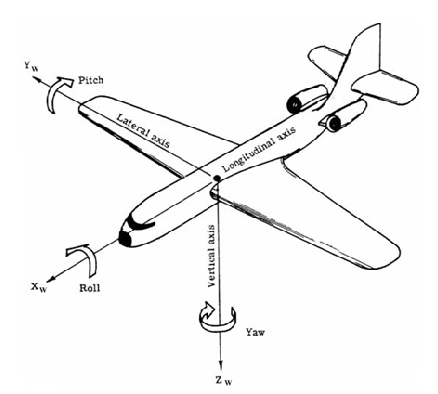
\includegraphics[scale=0.5]{pitchYawRoll.png}
    \caption{Movement directions for flying vehicles}
    \label{pitchYawRoll}
\end{figure}

\subsection{ROS And AT Commands}
ROS, or Robot Operating System, is an open-source, meta-operating system for your robot. People can write their own packages for all kinds of robots that other people
can reuse. This includes modules to control OpenCV, pathfinding etc. We explored options to control the \Ardrone with ROS but we came to the conclusion that the existing
module to control an \Ardrone with ROS does not work completely (but we could fix this ourselves) but also that it was way more complicated than what we actually needed. 
This is why we looked into other options such as AT Commands. \\

AT Commands are commands send to ports over the network telling the \Ardrone what to do directly. The \Ardrone listens to some ports for these commands and sends the 
navigation data and the video stream data back to the application using different ports. This is the most direct manner to control the \Ardrone and we were always able
to have the \Ardrone take off and land without problems by sending the take off and land commands. However, while sending commands to the \Ardrone was really easy, decoding
the navigation data and the video stream was not. We therefor decided to check out the Software Development Kit. Writen and documentated by the Parrot team itself. 

\subsection{Software Development Kit}
The Software Development Kit (SDK) did not came with it's documentation attached. We strangely found the documentation by clicking on a link in a remote part of the 
\Ardrone developer forum and it helped us a great deal. \\

The SDK is completely written in the programming language C. It allows you to use those features of the \Ardrone you want (or had time to implement). Figure \ref{mainloop}
shows us what we need to implement ourselves. We decided to grab an example provided by the SDK and modify this to our need. What we had to rewrite were:
\begin{itemize}
    \item The main initiation, update and close functions of the application. This is were we later would be sending the movement commands
    \item The navigation data processing functions. This had a seperate thread, especially to fetch the navigation data from the drone.
    \item The video stage functions. The SDK has a complete pipeline that receives, checksummes and processes the whole image. Just like the navigation data example
this ran on it's own seperated thread. It uses GTK (the standard C library for GUI's). 
\end{itemize}
This was rather complex C, and a lot of it we did not understand (both the example and the code in the SDK). So we decided to extend C with Python.

\begin{figure}[h!]
    \centering
        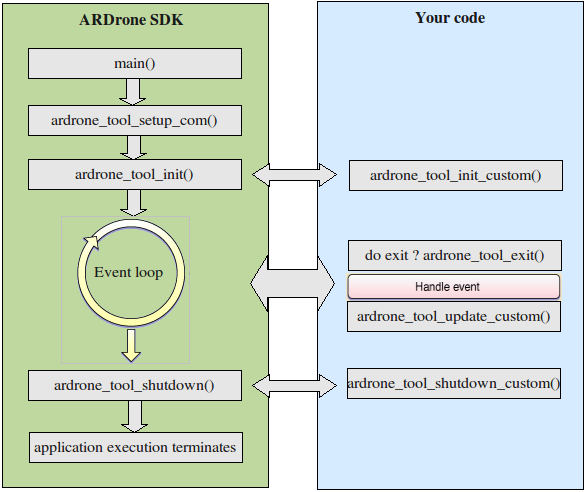
\includegraphics[scale=0.6]{mainloop.png}
    \caption{The application life cycle (picture from \href{https://projects.ardrone.org/embedded/ardrone-api/index.html}{\Ardrone API Webpage})}
    \label{mainloop}
\end{figure}

\subsection{Extending C With Python}
After we were able to safe an image frame to a file in C we could have Python read the file, process it, and send movements commands back to C. The main functions 
that took care of the initiation, updating and closing of the application instantiated and closed Python as well as updated Python. When C updated Python it supplied
Python with a tuple consisting of the frame counter (to retrieve the frame image) and the navigation data, and Python returned pitch, yaw, roll and gaz values (or something
to indicate that the application should exit). \\

While one might think that we decided to stick with the slowest manner to send the frame data from C to Python, it is not as bad as one would expect. Because each frame is
saved we could playback a run in which we flew with the \Ardrone and debug it completely and accurately. Later, we even saved the navigation data so we would be able to 
get an identical, simulated stream of information that was not actually send by the drone but rather read from file. This allowed us to easily debug any run and test 
probable solutions without flying with the \Ardrone over and over again. \\

Another something special we did with Python was using OpenCV. OpenCv can be used with Python quite easily, albeit some basic functions did not work even though everything
indicated it should be working, we were quite happy with it. \\

While it was not part of our direct goals, the bridge from the SDK written in C to our code written in Python using only one function that transfer all the necessary
data is something we expect could prove to be quite useful to other people as well. 


























